\blindtext\chapter{Composition of e-Learning Web Services in SOA}
\blindtext  \cite{com, com2}.
\section{e-Learning web Services}
\blindtext
\begin{itemize}
 \item Registration Service
\item Computer Programming Lectures service (Textual Narratives)
\item  Computer Programming Lectures service (Multimedia Narratives)
\item Online Examination Service
\end{itemize}

\begin{table}
 \begin{center}
 \caption{2nd Sample Table}
 \begin{tabular}{|c|c|}
 \hline
 B.Tech & CSE\\
 \hline
 M.Tech & ECE\\
 \hline
 Ph.D & EIE\\
 \hline 
 \end{tabular}
 \end{center}
\end{table}

\subsection{Registration Service}
Registration Service is the service to check whether a user, going to utilize the service is authorized user or not. If user is already registered
then he/she is allowed to avail the services otherwise, he/she is provided with 'register service' where he/she has to register first to access the services. This registration service 
has two functions 'Login' and 'Register'. Login method is to get into the system after successfull authentication such as login ID 
and 'Register method' is to register a user if he/she is not already the member of e-Learning system. (Figure.8)   

\begin{table}
 \begin{center}
 \caption{3rd Sample Table}
 \begin{tabular}{|c|c|}
 \hline
 B.Tech & CSE\\
 \hline
 M.Tech & ECE\\
 \hline
 Ph.D & EIE\\
 \hline 
 \end{tabular}
 \end{center}
\end{table}

%\begin{figure}[h!]
 %\centering
 %\includegraphics[width=16cm,height=13cm]{Register_Service_function_invoke.jpg}
 % Register_Service_function_invoke.jpg: 1024x768 pixel, 96dpi, 27.09x20.32 cm, bb=
%\caption{Registeration Service Invocation}
%\end{figure}
%\end{comments}

\subsection{Computer Programming Service (Textual Narratives)}
Computer Programming Lectures service (textual nrration) is service which provides the facility of downloading lectures in doc and 
pdf form. This service can only be accessed if the user is authorized by the system (Figure.9). 

\begin{table}
 \begin{center}
 \caption{4th Sample Table}
 \begin{tabular}{|c|c|}
 \hline
 B.Tech & CSE\\
 \hline
 M.Tech & ECE\\
 \hline
 Ph.D & EIE\\
 \hline 
 \end{tabular}
 \end{center}
\end{table} 
%\begin{figure}[h!]
% \centering
% \includegraphics[width=16cm,height=13cm]{CP_Service_main.JPG}
 %% CP_Service_main.JPG: 1024x768 pixel, 96dpi, 27.09x20.32 cm, bb=
 %\caption{Computer Programming Service}
%\end{figure}


\subsection{Computer Programming Service (Multimedia Narratives)}
Computer Programming Lectures service (Multimedia Narratives) is the service which provides the facility of downloading audio/video lectures
 This service can only be accessed if the user is authorized by the system and the client system is having the authorized player of the files. 
 
 \begin{table}
 \begin{center}
 \caption{5th Sample Table}
 \begin{tabular}{|c|c|}
 \hline
 B.Tech & CSE\\
 \hline
 M.Tech & ECE\\
 \hline
 Ph.D & EIE\\
 \hline 
 \end{tabular}
 \end{center}
\end{table} 
\subsection{Online Examination Service}
Online examination is examination system in which user can give the exam at his own pace limited by the system.
Online examination service is basis of the online certification of courses. On-line examination service is used to check the ability 
of a user in computer programming. As soon as user gets authorized he/she can access this service and can attempt questions online through the examination
 process. After the successful submission of examination answering, the user will get the result immediately (Figure. 10). 
 
 \begin{table}
 \begin{center}
 \caption{6th Sample Table}
 \begin{tabular}{|c|c|}
 \hline
 B.Tech & CSE\\
 \hline
 M.Tech & ECE\\
 \hline
 Ph.D & EIE\\
 \hline 
 \end{tabular}
 \end{center}
\end{table} 
%\begin{figure}[h!]
% \centering
% \includegraphics[width=16cm,height=13cm]{Exam_Service_main.jpg}
 % Exam_Service_main.jpg: 1024x768 pixel, 96dpi, 27.09x20.32 cm, bb=0 0 768 576
 %\caption{Online Exam Service}
%\end{figure}



\section{e-Learning Web Services: Publish and Subscription Methodology}
e-Learning system composed of number of services, some of them are primary web services and some are secondary as per need. Primary 
service are used for the coordination of other services as UDDI service and  compatibility checking service. Secondary services 
include fully functioned stand alone services as registration service, online examination service, etc.

\begin{table}
 \begin{center}
 \caption{7th Sample Table}
 \begin{tabular}{|c|c|}
 \hline
 B.Tech & CSE\\
 \hline
 M.Tech & ECE\\
 \hline
 Ph.D & EIE\\
 \hline 
 \end{tabular}
 \end{center}
\end{table}
\subsection{Publishing e-Learning Web Services into UDDI}
The e-Learning system, for local UDDI, is prepared and presented through the web portal (Figure 11) .UDDI service in Microsoft Web Server 2008 is configured.  Registration service, Computer 
Programming Service (Texual Narratives), Computer Programming Service (Multimedia narratives) and online examination services are published on different
systems and registered with service provider's name to UDDI by publish service of UDDI \cite{support, uddi, service}. UDDI Service 
requires Provider's name and the service’s WSDL file for it’s publication in UDDI registry. The process is shown in figure.11; 12; 13.

\begin{table}
 \begin{center}
 \caption{8th Sample Table}
 \begin{tabular}{|c|c|}
 \hline
 B.Tech & CSE\\
 \hline
 M.Tech & ECE\\
 \hline
 Ph.D & EIE\\
 \hline 
 \end{tabular}
 \end{center}
\end{table}

% \begin{figure}[h!]
% \centering
% \includegraphics[width=16cm,height=13cm]{uddi_home_interface.jpg}
%\caption{UDDI home Interface}
 % uddi_home_interface.jpg: 1024x768 pixel, 96dpi, 27.09x20.32 cm, bb=0 0 768 576
%\end{figure}
%\begin{figure}[h!]
% \centering
% \includegraphics[width=16cm,height=13cm]{provider_interface.jpg}
%\caption{UDDI Provider Interface}
 % provider_interface.jpg: 1022x544 pixel, 96dpi, 27.04x14.39 cm, bb=0 0 767 408
%\end{figure}
%\begin{figure}[h!]
% \centering
 %\includegraphics[width=16cm,height=13cm]{uddi_add_service.jpg}
 % uddi_add_service.jpg: 1019x683 pixel, 96dpi, 26.96x18.07 cm, bb=0 0 764 512
 %\caption{UDDI Add Service Interface}
%\end{figure}
\begin{itemize}
 
\item On the configured UDDI Services home page 'Publish' button is clicked. The configured UDDI open the page 'My UDDI'.
\item On the 'My UDDI' page, the Providers tab is clicked and a number of options is shown through the menu.
\item On the Providers tab, 'Add Provider' is chosen to be clicked. The 'My UDDI' (New Provider Name) page appears in the browser for 
providing option to add new providers name. 
\item On the 'My UDDI' (New Provider Name) page, the Edit button 'under actions' is chosen to be clicked. The name is required to be edit. The 'Name' text button
appears.
\item In the 'Name' textbox,  New WebService is typed, and then Update button is clicked. The 'My UDDI' (NewWebService) page appears again in the browser with all the added information.
\item 'My UDDI' (NewWebService) page provides the services, that is required to be checked then Add Service is another option that is avilable
in this option. It is clicked. A number of options are again available.
\item Under Actions, option Edit is selected to be clicked, the textbox of 'Name' is filled with service 1. The next step is to update 
the information by clicking Update.
\item  On the 'My UDDI' New Service 1 page, Bindings tab appears with a number of options.
\item Add Binding tab is activated by clicking.
\item Again the 'My UDDI' NewWebService Service1 http://'' page, Edit button is chosen to be clicked. The Access Point textbox appears.
\item In the Access Point textbox, the URL of the services composed is typed. Update button is clicked for required updation 
$http://computer\_name/Service1.asmx$
In the URL, computer\_name is replaced with the name of the server that hosts the Web service. $``http://localhost''$ in the URL should not be used..
\item On the UDDI Services page, the 'Instance Info' tab is clicked.
\item Again, on the Instance Info tab, Add Instance Information is checked out. 
\end{itemize}

\begin{table}
 \begin{center}
 \caption{9th Sample Table}
 \begin{tabular}{|c|c|}
 \hline
 B.Tech & CSE\\
 \hline
 M.Tech & ECE\\
 \hline
 Ph.D & EIE\\
 \hline 
 \end{tabular}
 \end{center}
\end{table}

The client system searches the required services and their location, other details of services which are required to use those 
services are obtained. These services required to be composed, are available so that a learner or visitor to our 
e-Learning system can get the access of these services in a user friendly manner. 
\subsection{Searching e-Learning Web Services in UDDI}
Web services can be searched in UDDI by using the keywords. 'Search' function of UDDI returns the service provider name, Service location 
with other details, through it’s WSDL detail (Figure. 14).
\begin{figure}[h!]
 \centering
 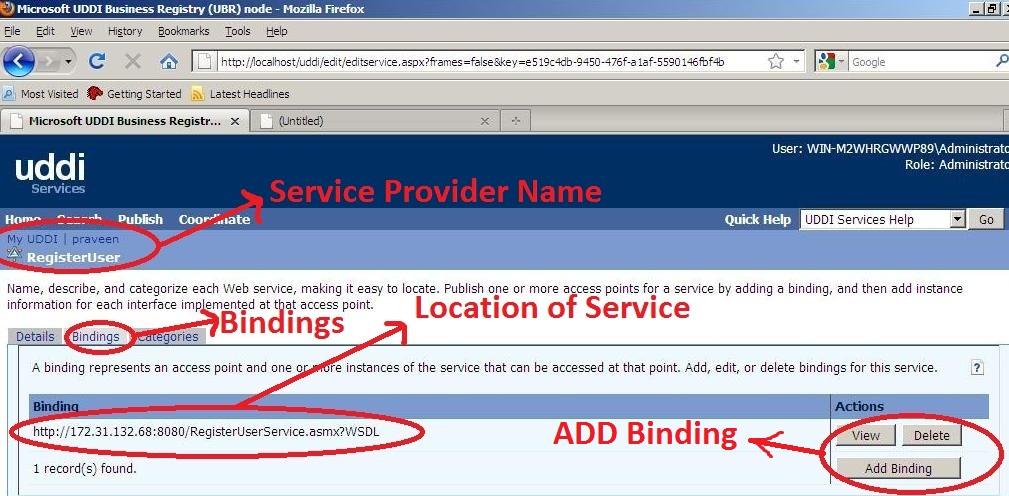
\includegraphics[width=16cm,height=13cm]{uddi_service_binding_interface.jpg}
 % uddi_service_binding_interface.jpg: 1009x496 pixel, 96dpi, 26.70x13.12 cm, bb=0 0 757 372
 \caption{UDDI Service Binding Interface}
\end{figure}

\begin{table}
 \begin{center}
 \caption{10th Sample Table}
 \begin{tabular}{|c|c|}
 \hline
 B.Tech & CSE\\
 \hline
 M.Tech & ECE\\
 \hline
 Ph.D & EIE\\
 \hline 
 \end{tabular}
 \end{center}
\end{table}
\section{e-Learning  Web  Services: Composition Technique}
To provide learning facility to the user we considered three types of e-Learning services
\begin{itemize}
\item Computer programming Service (Textual Narratives)
\item Computer programming Service (Multimedia Narratives)
\item Online Examination Service

\end{itemize}

\begin{table}
 \begin{center}
 \caption{11th Sample Table}
 \begin{tabular}{|c|c|}
 \hline
 B.Tech & CSE\\
 \hline
 M.Tech & ECE\\
 \hline
 Ph.D & EIE\\
 \hline 
 \end{tabular}
 \end{center}
\end{table}
\begin{figure}[h!]
 \centering
 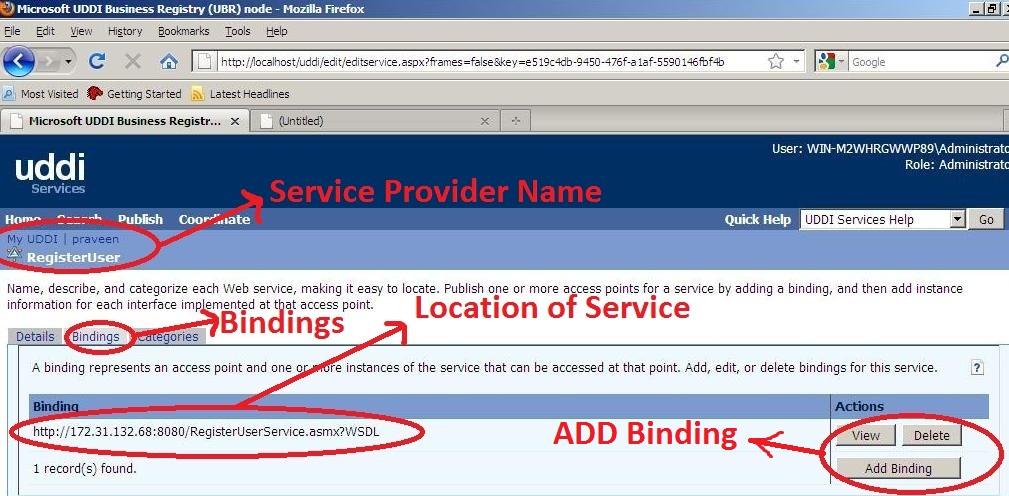
\includegraphics[width=16cm,height=13cm]{uddi_service_binding_interface.jpg}
 % uddi_service_binding_interface.jpg: 1009x496 pixel, 96dpi, 26.70x13.12 cm, bb=0 0 757 372
 \caption{UDDI Service Binding Interface}
\end{figure}
Each of these services is stand alone and totally independent from others. Besides these services, there are other services 
like registration service, this is also stand alone and independent service registration service. Registration service can be composed to every of the service mentioned above. 


\begin{table}
 \begin{center}
 \caption{12th Sample Table}
 \begin{tabular}{|c|c|}
 \hline
 B.Tech & CSE\\
 \hline
 M.Tech & ECE\\
 \hline
 Ph.D & EIE\\
 \hline 
 \end{tabular}
 \end{center}
\end{table}
\subsubsection{Composition of Computer Programming Service (Textual Narratives) with Registration Service}
\blindtext
\begin{figure}[h!]
 \centering
 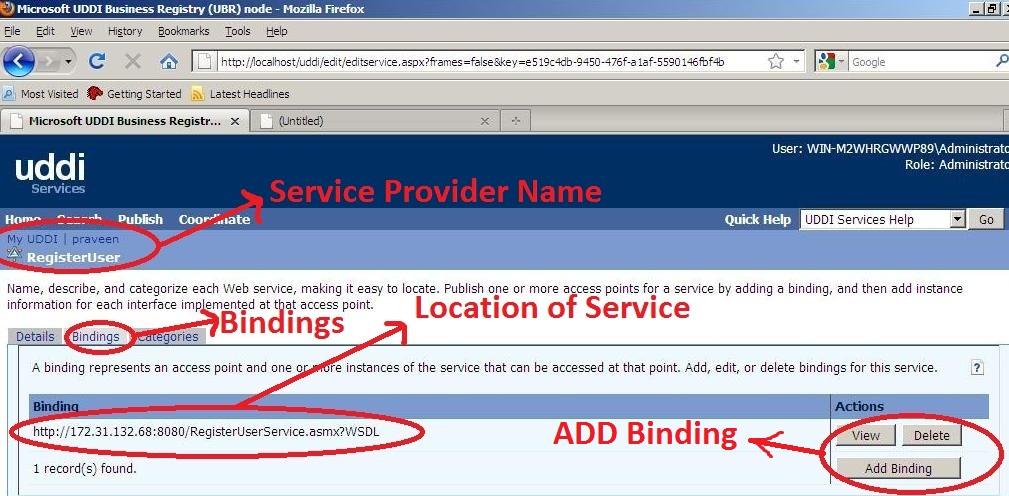
\includegraphics[width=16cm,height=13cm]{uddi_service_binding_interface.jpg}
 % uddi_service_binding_interface.jpg: 1009x496 pixel, 96dpi, 26.70x13.12 cm, bb=0 0 757 372
 \caption{UDDI Service Binding Interface}
\end{figure}

\begin{table}
 \begin{center}
 \caption{13th Sample Table}
 \begin{tabular}{|c|c|}
 \hline
 B.Tech & CSE\\
 \hline
 M.Tech & ECE\\
 \hline
 Ph.D & EIE\\
 \hline 
 \end{tabular}
 \end{center}
\end{table}
\subsubsection{Computer Programming Service (Multimedia Narratives) Composition with Registration Service}
\Blindtext
\begin{figure}[h!]
 \centering
 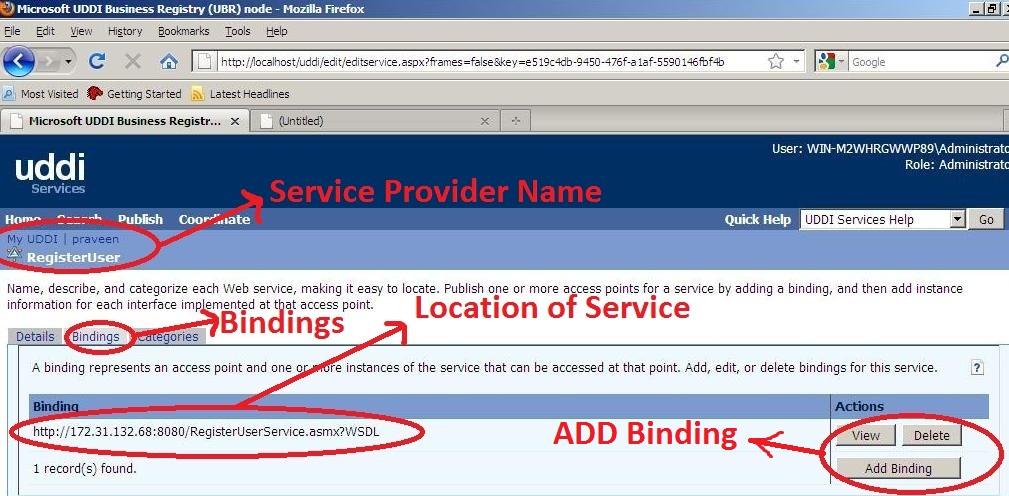
\includegraphics[width=16cm,height=13cm]{uddi_service_binding_interface.jpg}
 % uddi_service_binding_interface.jpg: 1009x496 pixel, 96dpi, 26.70x13.12 cm, bb=0 0 757 372
 \caption{UDDI Service Binding Interface}
\end{figure}

\begin{table}
 \begin{center}
 \caption{14th Sample Table}
 \begin{tabular}{|c|c|}
 \hline
 B.Tech & CSE\\
 \hline
 M.Tech & ECE\\
 \hline
 Ph.D & EIE\\
 \hline 
 \end{tabular}
 \end{center}
\end{table}
\subsubsection{Online Examination Service  Composition with Registration Service}
\Blindtext
\begin{figure}[h!]
 \centering
 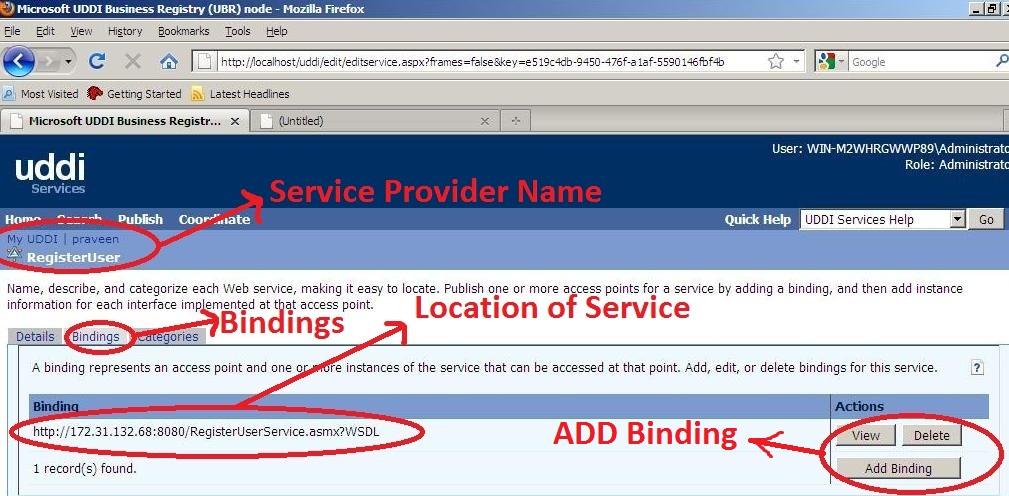
\includegraphics[width=16cm,height=13cm]{uddi_service_binding_interface.jpg}
 % uddi_service_binding_interface.jpg: 1009x496 pixel, 96dpi, 26.70x13.12 cm, bb=0 0 757 372
 \caption{UDDI Service Binding Interface}
\end{figure}

\begin{table}
 \begin{center}
 \caption{15th Sample Table}
 \begin{tabular}{|c|c|}
 \hline
 B.Tech & CSE\\
 \hline
 M.Tech & ECE\\
 \hline
 Ph.D & EIE\\
 \hline 
 \end{tabular}
 \end{center}
\end{table}
\subsection{e-Learning Web Service Composition Algorithm}
Web services composition synchronization is achieved from services compatability and their on-the-fly binding from the option like'Add References'. When Registration service gets composed with computer programming service and online examination service the method makes application of the value of service for storing in a variable. 
After the successful completion of registration service the value stored in the variable is checked.     

\begin{algorithm*}[!htb]
\caption{Service Composition Method: A Sample}
\begin{code}
\uln \>\ubegin\\
\uln \>\>  $Get\ service\ choice\ from\ user$\\
\uln \>\>\> $Save\ choice\ into\ a\ variable\ 'var'$ \\
\uln \>\> $Call \ Login \ Service \ with\ a \ argument\ of \ saved \ variable\ (var)$\\
\uln \>\>\> $Do\ Login\ (validation)$\\
\uln \>\>\>\uif $user\ is\ valid$) \uthen\\
\uln \>\>\>\> $check\ variable$\ (var)\\
\uln \>\>\>\> $call\ service\ which\ refer\ to\ (var) $)\\
\uln \>\>\>\> $Get\ the\ result\ of\ service  $\\
\uln \>\>\>\> $Return\ result$\\
\uln \>\>\>\uelse  $Return\ error\ to\ caller\ of\ Login\ Function$  \\
\uln \>\uend\\ 
\end{code}
\label{alg:dfs}
\end{algorithm*}


\section{e-Learning Web Portal: e-Learning Web Services and their Composition}
The e-Learning portal under consideration provides three application that make use of the programming  services to the end user computer programming service in doc, pdf document downloads,
in audio/video file downloads and online examination to the end user. These functions are simple application through GUI in the stand alone
mode in a client service architecture. However, the access and composition of these services for different application from different nodes
at different logical locations calls for capacity building in distributed system architecture and compatability governance in service oriented architecture. 
 \begin{figure}[h!]
 \centering
 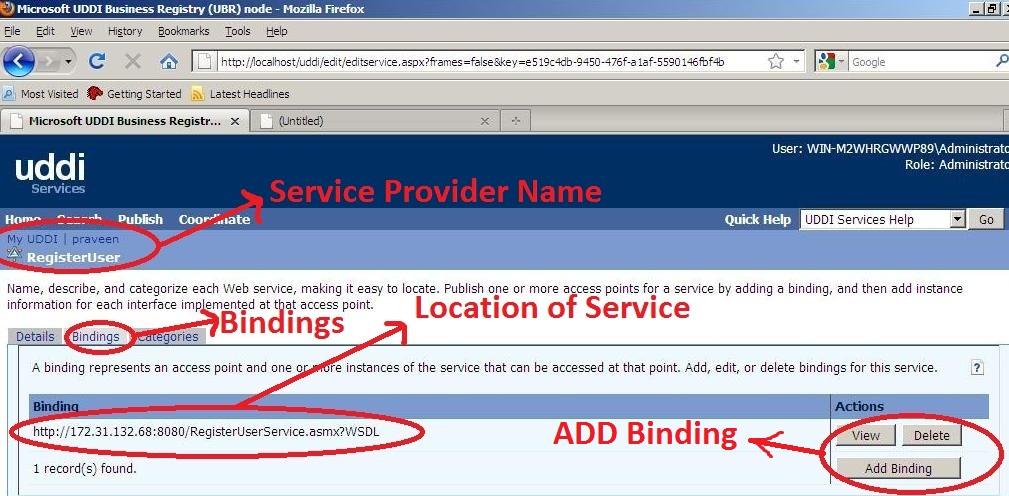
\includegraphics[width=16cm,height=13cm]{uddi_service_binding_interface.jpg}
 % uddi_service_binding_interface.jpg: 1009x496 pixel, 96dpi, 26.70x13.12 cm, bb=0 0 757 372
 \caption{UDDI Service Binding Interface}
\end{figure} 
\subsection{Home page of the e-Learning web portals}
Home page shows the sample services provided by e-Learning web portal. The services may be identified and accessed by the identity of service name. The functionality and implementation  of services are hidden from the user and provides only output by interactive GUI to the user. Home Page shows links to all services availlable
in the designed e-Learning web portal. By clicking these link user can access the complete functioality of composite services which are unknown to him/her earlier.\par
Home Page contains three links for each services (Computer Programming Service, Audio/video service and Online Examination service).
The user can select any one of the service and can get composed service with Registration service (Figure. 17) with one of the available services.
\begin{figure}[h!]
 \centering
 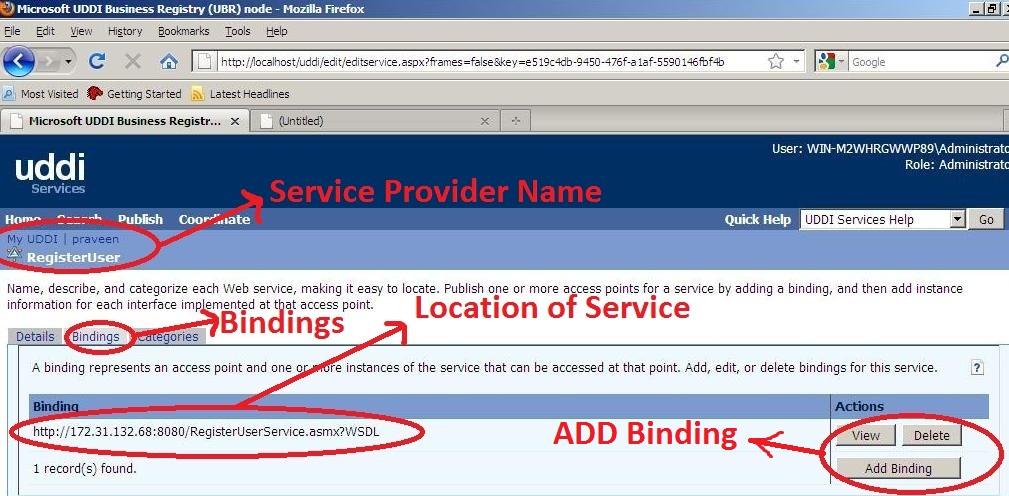
\includegraphics[width=16cm,height=13cm]{uddi_service_binding_interface.jpg}
 % uddi_service_binding_interface.jpg: 1009x496 pixel, 96dpi, 26.70x13.12 cm, bb=0 0 757 372
 \caption{UDDI Service Binding Interface}
\end{figure} 
%\begin{figure}[h!]
% \centering
% \includegraphics[width=16cm,height=13cm]{Application_home.jpg}
 % Application_home.jpg: 1024x768 pixel, 96dpi, 27.09x20.32 cm, bb=0 0 768 576
% \caption{Home page of the e-Learning web portal}
%\end{figure}
\subsection{Login page of the e-Learning Web Portal}
When user click on any of the service links in the Home page, Login Page is presented on the monitor. If the user is not registered then he/she has to get registered first. for that he/she has to 
click on the register link (Figure.18) as shown.
\begin{figure}[h!]
 \centering
 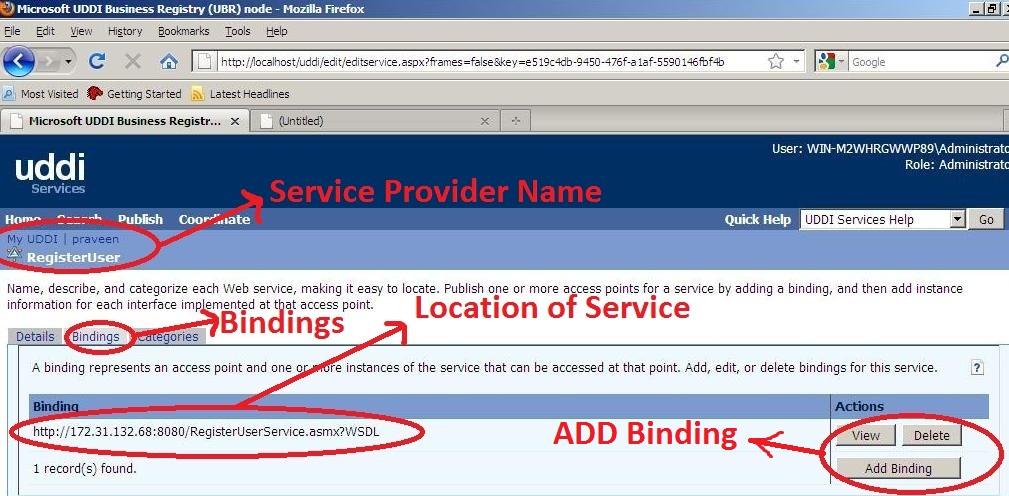
\includegraphics[width=16cm,height=13cm]{uddi_service_binding_interface.jpg}
 % uddi_service_binding_interface.jpg: 1009x496 pixel, 96dpi, 26.70x13.12 cm, bb=0 0 757 372
 \caption{UDDI Service Binding Interface}
\end{figure}
%\begin{figure}[h!]
% \centering
% \includegraphics[width=16cm,height=13cm]{Application_login.jpg}
 % Application_login.jpg: 1024x768 pixel, 96dpi, 27.09x20.32 cm, bb=0 0 768 576
 %\caption{Login Page}
%\end{figure}
\subsection{Registration Page of the e-Learning Web Portal}
If user is already registered then he can access services through login process. If the user is not registered  then he/she has to register first by
filling the Registarion page. He/She has to fill the required fields and submit for registration. 
The user is allowed to access other services which are composed with 
Registration service. Login service itself is automatically invoked when the user chooses to click on any service link (Figure. 19).
\begin{figure}[h!]
 \centering
 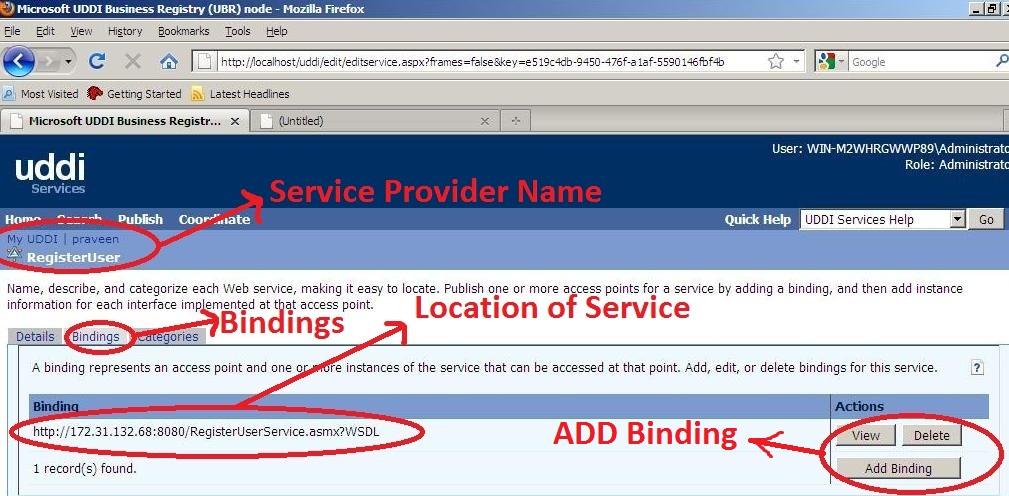
\includegraphics[width=16cm,height=13cm]{uddi_service_binding_interface.jpg}
 % uddi_service_binding_interface.jpg: 1009x496 pixel, 96dpi, 26.70x13.12 cm, bb=0 0 757 372
 \caption{UDDI Service Binding Interface}
\end{figure}
%\begin{figure}[h!]
% \centering
 %\includegraphics[width=16cm,height=13cm]{Application_register.jpg}
 % Application_register.jpg: 1024x768 pixel, 96dpi, 27.09x20.32 cm, bb=0 0 768 576
 %\caption{Register Page}
%\end{figure}
\subsection{Programming Service page the of e-Learning Web Portal}
The e-Learning link on the Home Page provides the Registration service for user authentication. If the user is authorized then Programming Service Page offers the downloading-services from where user can download the lectures in doc or pdf format.
Programming Service (textual/Multimedia narratives) is also similar in capacity to Programming Service for the lectures in doc or pdf format (Figure. 20) 
\begin{figure}[h!]
 \centering
 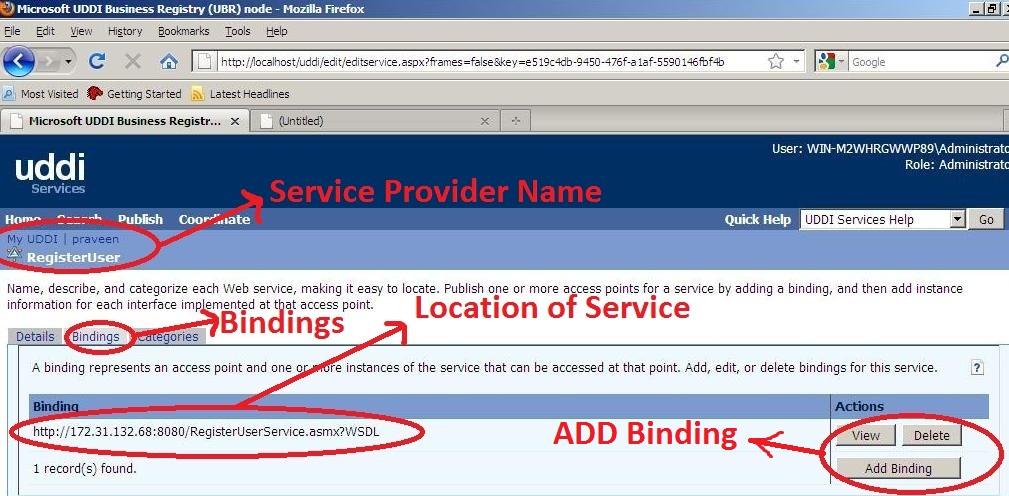
\includegraphics[width=16cm,height=13cm]{uddi_service_binding_interface.jpg}
 % uddi_service_binding_interface.jpg: 1009x496 pixel, 96dpi, 26.70x13.12 cm, bb=0 0 757 372
 \caption{UDDI Service Binding Interface}
\end{figure}

\subsection{Online Examination Page of e-Learning web portal}
Online Exam page gets opened from the link on Home page. The service first invokes Login page on the monitor. The user is already
registered then the user can avail the examination service. Otherwise the user has to register himself/herself first (Figure.21).
\begin{figure}[h!]
 \centering
 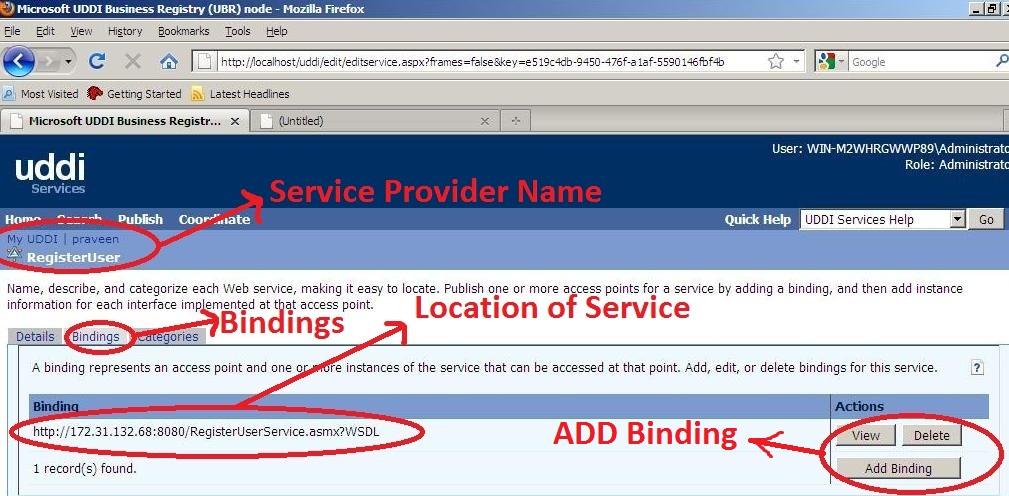
\includegraphics[width=16cm,height=13cm]{uddi_service_binding_interface.jpg}
 % uddi_service_binding_interface.jpg: 1009x496 pixel, 96dpi, 26.70x13.12 cm, bb=0 0 757 372
 \caption{UDDI Service Binding Interface}
\end{figure}